\documentclass[10pt,a4paper]{article}
\usepackage[latin1]{inputenc}
\usepackage[spanish]{babel}
\usepackage{amsmath}
\usepackage{amsfonts}
\usepackage{amssymb}
\usepackage{graphicx}
\usepackage[left=2cm,right=2cm,top=2cm,bottom=2cm]{geometry}
\author{Jorge Marroqu�n}
\begin{document}

\begin{center}
        \huge{Parcial \#1} \\
\end{center}
\begin{center}
        \textbf{Nombre: }Jorge Armando Marroqu�n Ochoa\\
        \textbf{Carnet: }2018358\\
        \textbf{Correo: }marroquin181358@unis.edu.gt\\
\end{center}

\section{Ejercicio \#1} 
\begin{center}
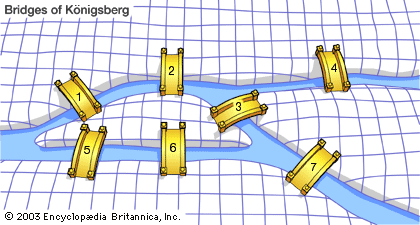
\includegraphics[width=8cm]{bridges.png}
\end{center}

\begin{itemize}
        \item{\textbf{Nodos: }$\{1,2,3,4,5,6\}$}
        \item{\textbf{V�rtices: }
\begin{tabular}{p{0cm} c}
    $$
    \left\{
        \begin{bmatrix}
            \langle 1,2 \rangle & \langle 1,3 \rangle & \langle 1,4 \rangle \\
            \langle 1,5 \rangle & \langle 1,6 \rangle & \langle 2,3 \rangle \\
            \langle 2,4 \rangle & \langle 2,5 \rangle & \langle 2,6 \rangle \\
            \langle 3,4 \rangle & \langle 3,5 \rangle & \langle 3,6 \rangle \\
            \langle 3,7 \rangle & \langle 4,7 \rangle & \langle 5,6 \rangle \\
            \langle 5,7 \rangle & \langle 6,7 \rangle & \\
        \end{bmatrix}
    \right\}
$$

\end{tabular}        
        } \\  \\  \\ \\ \\ \\
\end{itemize}


\section{Ejercicio \#2}
\[
        \sum_{i=1}^{n}{i}=\frac{n(n+1)}{2}
\]
\begin{enumerate}
\item {\textbf{Caso Base:}}\\
\begin{itemize}
        \item{\[ \sum_{i=1}^{1}{i}=\frac{1(1+1)}{2} \]}
        \item{\[ \sum_{i=1}^{1}{i}=\frac{1(2)}{2} \]}
        \item{\[ \sum_{i=1}^{1}{i}=\frac{2}{2} \]}
        \item{\[ \sum_{i=1}^{1}{i}= 1 \]}
\end{itemize}
\item {\textbf{Hip�tesis Inductiva:}}\\
\begin{itemize}
        \item{\[ \sum_{i=1}^{n+1}{i}=\frac{n(n+1)}{2} \]}
        \item{\[ \sum_{i=1}^{n+1}{i}=\frac{(n+1)((n+1)+1)}{2} \]}
        \item{\[ \sum_{i=1}^{n+1}{i}=\frac{(n+1)(n+2)}{2} \]}
        \item{\[ \sum_{i=1}^{n+1}{i}=(n+1)\frac{(n+2)}{2} \]}
        \item{\[ \sum_{i=1}^{n+1}{i}=(n+1)(\frac{n}{2}+1) \]}
        \item{\[ \sum_{i=1}^{n+1}{i}=\frac{n(n+1)}{2}+(n+1) \]}
        \item{\[ \sum_{i=1}^{n+1}{i}=\frac{n(n+1)2(n+1)}{2} \]}
        \item{\[ \sum_{i=1}^{n+1}{i}=\frac{(n+1)(n+2)}{2} \]}
        \item{\[ \sum_{i=1}^{n+1}{i}=\frac{(n+1)((n+1)+1)}{2} \]}
\end{itemize}

\end{enumerate}
\section{Ejercicio \#3}
\begin{itemize}
        \item{$ \frac{s(0) \otimes ( s(0) \oplus  s(0) )}{s(s(0))}$}
        \item{$ \frac{s(0) \otimes  s(s(0)) }{s(s(0))}$}
        \item{$ \frac{ s(s(0)) }{s(s(0))}$}
        \item{$ s(0)$}

\end{itemize}
\section{Ejercicio \#4}
\begin{center}
$a\oplus b = b\oplus a$
\end{center}
\begin{enumerate}
\item {\textbf{Caso Base:}}\\
\begin{itemize}
        \item{$0\oplus 0 = 0\oplus 0$}
        \item{$0 = 0$}
\end{itemize}

\item {\textbf{Hip�tesis Inductiva:}}\\

\begin{itemize}
        \item{$a = s(i)  y  b = s(j)$}
        \item{$s(i)\oplus b = b\oplus s(i)$}
        \item{$s(i \oplus b) = s(b \oplus i)$}
        \item{$s(i \oplus b) = s(i \oplus b)$ equivale a $s(i \oplus s(j)) = s(i \oplus s(j))$}

\end{itemize}
\end{enumerate}
\section{Ejercicio \#5}
\begin{center}
$((n\oplus n)\geq n) = s(o)$
\end{center}
\begin{enumerate}
\item {\textbf{Caso Base:}}\\
\begin{itemize}
        \item{$((1 + 1)\geq 1) = 1$}
        \item{$( 2 \geq 1) = 1$}
        \item{$((2 - 1)\geq 0) = 1$}
        \item{$1\geq 0 = 1$}
\end{itemize}

\item {\textbf{Hip�tesis Inductiva:}}\\

\begin{itemize}
        \item{$((s(i) \oplus (s(i))\geq (s(i)) = s(o)$}
        \item{$(s(s(i))\geq (s(i)) = s(i)$}
        \item{$(s(s(i)) \ominus (s(i))\geq o) = s(0)$}
        \item{$(s(i) \geq o) = s(o)$}

\end{itemize}
\end{enumerate}
\end{document}
